\section{CUDA IF2 Spatial Fitting Code}

	Below is the nascent CUDA code that will be expanded upon in future work. At present it only implements the core IF2 fitting algorithm and does not implement parametric bootstrapping nor produce forecasts.

	\lstinputlisting[style=Cppsty]{../../code/cuIF2/cuIF2.cu}

	Figure [\ref{cudatimeplot2}] shows the running times for parameter fitting as compared to IF2 and HMCMC.

	\begin{figure}[H]
        \centering
        \captionsetup{width=.8\linewidth}
        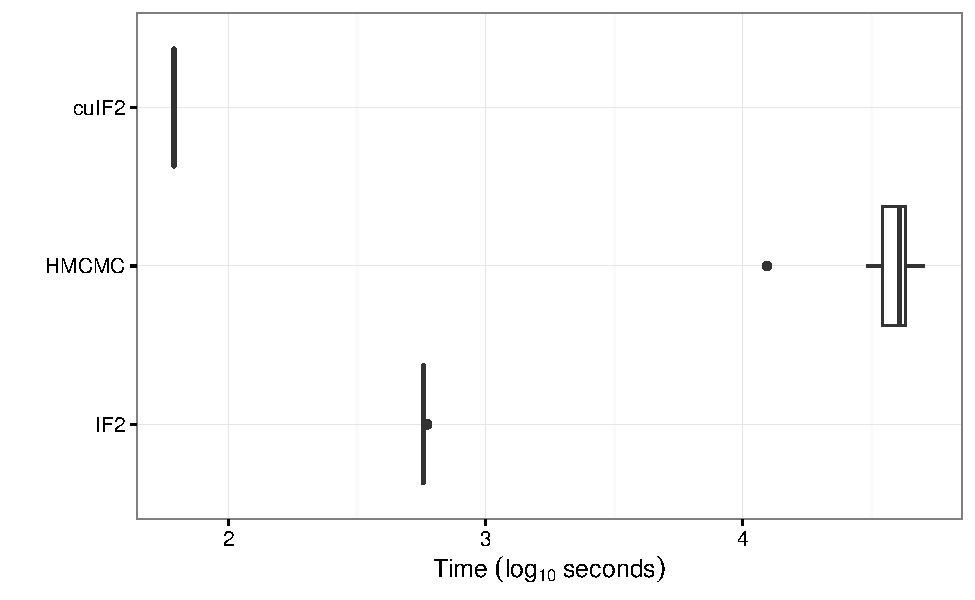
\includegraphics[width=0.8\textwidth]{./images/timeplot2.pdf}
        \caption{Running times for fitting the spatial SIR model to data. \label{cudatimeplot2}}
    \end{figure}

    The means from the data in Figure [\ref{cudatimeplot2}] are about $61.5$ seconds for \texttt{cuIF2}, $574$ seconds for IF2, and $38,800$ seconds for HMCMC. For \texttt{cuIF2} This is a speedup of over $9.33$x against IF2 and over $617$x against HMCMC.

